\section{Results}
\label{sec:results}

\subsection{Attenuation Refined Physical Reachability Under the Registered Obligations}

The formal audit recorded a closed argument for all eight registered proof items: one for each of the first five obligations in Section~\ref{sec:theorem}, the forward-simulation and trace-projection steps that rely on the sixth, and the exact one-dimensional corollary. The exact implementation then evaluated 393,750 one-dimensional models and 2,756,250 horizon checks without finding a child state outside its parent reachable set. This finite zero-violation result checked the executable semantics; the induction in Theorem~1, rather than the enumeration scale, establishes the conditional general result. The audit also retained a counterexample to the stronger same-request property instead of broadening the theorem.

The falsification runs exercised alternatives to the registered conditions. All 14 unsafe caveat, default, combiner, and semantic mutants produced counterexamples. Across the five preregistered seeds, the coupled MIMO and history-dependent runs found no registered violation in 720 MIMO horizon checks, 400 history horizon checks, and 8,854 child-trace membership checks; both widening controls were detected. Removing rewrite closure or the parent-admissible hold premise produced the two expected horizon-one counterexamples. Restoring the premises eliminated the registered violations while reaching every effect.

The common-subset comparison used only invariant resource identity, action inclusion, and a non-negative physical upper bound. Across 72 request pairs and 63 adapter/plant/horizon checks, \zonecap{}, pinned SINT, and the Dodson schema adapter had no decision or reachable-set mismatch in that shared scope. The Dodson path was a schema adapter rather than a reproduction of the complete system, and proof-specific dimensions were not assigned to either baseline. This comparison therefore bounds semantic compatibility; it does not establish implementation or performance superiority.

\subsection{Compilation Matched the Frozen Corpus and Rejected Widening}

The complete compiler corpus contained 58,968 cases: 42,120 derived from the CPwE matrix and 16,848 from the ENISA landside-signalling subgraph. The total comprised 4,536 valid source-plus-overlay combinations and 54,432 single-field mutations. The \zonecap{} compiler and separate table oracle agreed on every decision. Across 84 registered delegation edges, all 672 checks covering the eight authority dimensions passed.

Mutation, path, and provenance tests challenged the perfect agreement. The generated corpus killed all ten check-removal mutants, whereas six handwritten happy paths killed none. Four source-grant addition or removal probes changed the expected roots, descendants, case counts, conduits, and assets without failure. All 24 multi-conduit path cases, covering two paths without a direct grant at delegation depths 0--2, matched the oracle, all 32 localized widening attempts were rejected, and 22 boundary sanity cases produced their expected outcomes. Fig.~\ref{fig:compiler-results} separates corpus scale from these decisive controls. The controls test disabled or misrouted checks, but they do not independently validate the shared human interpretation of the source tables.

On fully expressible subsets, the OPC UA role, PLC ABAC, and pinned-SINT projections each agreed with their corresponding oracle decisions. On the full corpus, however, the projections left 40,824, 18,144, and 28,728 mutations unrestricted, respectively, because those cases involved unrepresented dimensions. These counts measure schema coverage under the registered projection; they are not false-allow rates for deployed OPC UA, ABAC, or SINT systems. Table~\ref{tab:policy-baselines} makes this comparison boundary explicit. \zonecap{}'s measured distinction is the joint representation of the registered fields and their connection to the refinement obligations.

\begin{table*}[t]
\caption{Policy-projection scope and full-corpus outcome. ``Exact categories'' counts the registered mutation categories represented without projection loss. Fair-subset cases comprise the 4,536 valid requests plus 4,536 cases per exactly represented category, and agreement is reported only on that subset; the \zonecap{} row is the main compiler--oracle comparison. Unrestricted mutations are full-corpus cases a projection allowed because it did not represent the mutated dimension; for the pinned SINT profile, 3,024 of the 31,752 cases outside its fair subset were still denied by a partial parameter check. These counts are not measured deployed-product error rates.}
\label{tab:policy-baselines}
\centering
\footnotesize
\setlength{\tabcolsep}{7pt}
\begin{tabular}{@{}lrrrr@{}}
\toprule
System/profile & Exact categories (of 12) & Fair-subset cases & Fair-subset agreement & Unrestricted mutations \\
\midrule
\zonecap{} & 12 & 58,968 & 100\% & 0 \\
OPC UA role projection & 3 & 18,144 & 100\% & 40,824 \\
PLC ABAC projection & 8 & 40,824 & 100\% & 18,144 \\
Pinned SINT profile & 5 & 27,216 & 100\% & 28,728 \\
\bottomrule
\end{tabular}
\end{table*}

\begin{figure*}[t]
\centering
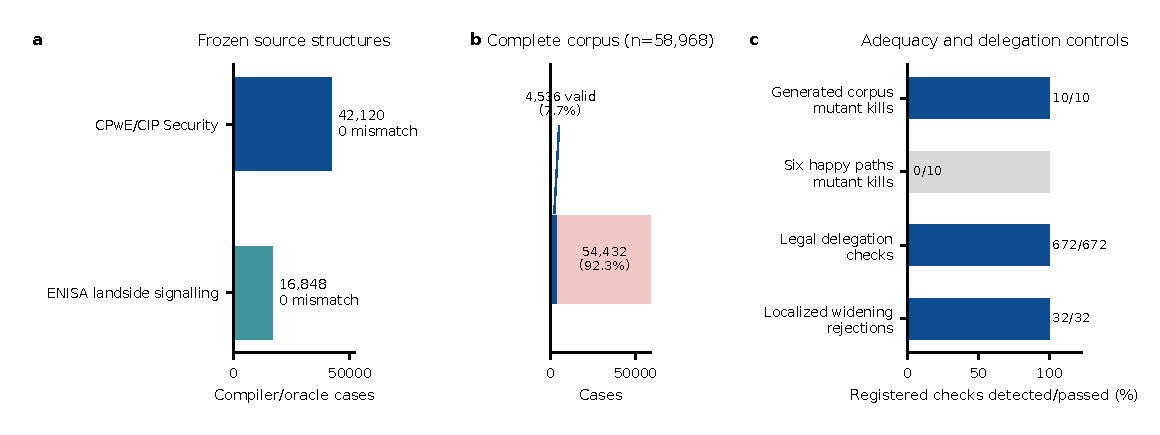
\includegraphics[width=\textwidth]{figures/generated/fig03_compiler_results}
\caption{Compiler agreement, corpus composition, and decisive controls. (a) Exact case counts from the two frozen source structures; the compiler and separate table oracle disagreed on none of them. (b) The complete 58,968-case corpus contains every 4,536 valid source-plus-overlay combination and 54,432 single-field mutations. (c) The generated corpus killed all 10 check-removal mutants, whereas six handwritten happy paths killed none; all 672 legal delegation-dimension checks passed and all 32 localized widening attempts were rejected. These seedless counts validate the frozen encoding and implementation checks, not the shared human interpretation of the source tables.}
\label{fig:compiler-results}
\end{figure*}

\subsection{Five Runtime Effects Preserved the Bounded Actuation-Event Refinement}

The main runtime run evaluated all 58,968 frozen one-request cases and one five-step composed trace for each of the 4,536 valid cases. Every effect was reached. No registered authority, parent-realizability, trace-inclusion, stutter, effect-order, or bounded-deadlock violation occurred, and all five negative-control mutants were detected. These observations apply to the registered actuation-event semantics, in which no-output decisions do not advance the plant.

The exhaustive study enumerated 492,156 words and 492,030 transitions through horizon five over 126 scopes. It covered all 25 effect bigrams and all 125 trigrams without a registered violation or deadlock, and it killed all three sequence-triggered mutants. In contrast, one named path per scope covered only four bigrams and three trigrams and killed none of those mutants. Exhaustive enumeration therefore tested interaction orders missed by individually effect-complete paths; it does not imply unbounded or asynchronous progress.

Replacing \texttt{ATTENUATE}, \texttt{REWRITE}, and \texttt{DEFER} with no-output denial preserved zero registered safety violations but removed behavior the frozen semantics treated as recoverable or safely corrected. Deny-only blocked 13,608 rewrite steps, or 16.67\% of the 81,648 constructed policy steps and 60\% of the constructed safe-service opportunities, and removed 9,072 attenuation or deferral recovery decisions. These fractions characterize the generated corpus, not an industrial workload distribution. Fig.~\ref{fig:runtime-results} separates effect incidence, interaction-order coverage, and physical-output loss.

\begin{figure*}[t]
\centering
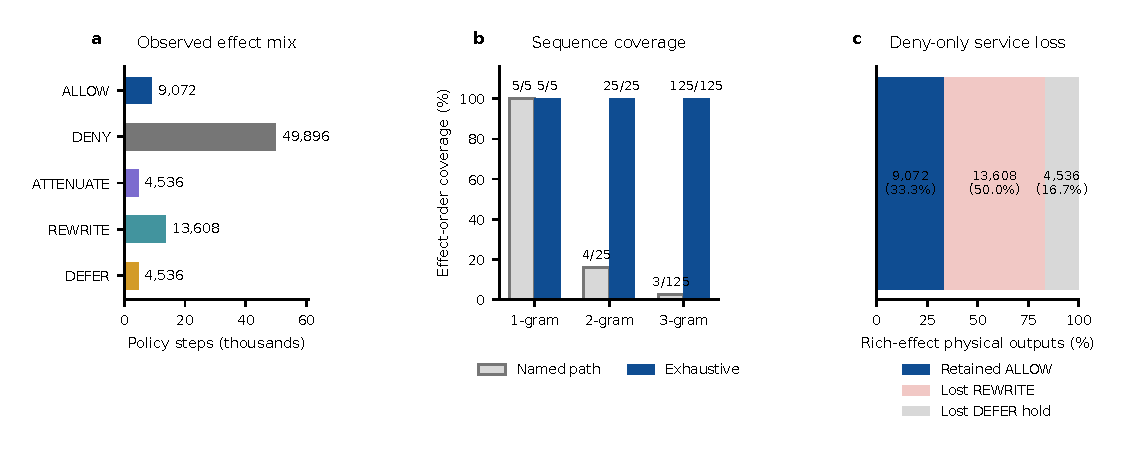
\includegraphics[width=\textwidth]{figures/generated/fig04_runtime_results}
\caption{Runtime-effect incidence, sequence coverage, and deny-only service loss. (a) Counts of the five observed effects over all 81,648 registered policy steps. (b) One named path per scope covered all five effects individually but only 4 of 25 effect bigrams and 3 of 125 trigrams; exhaustive enumeration through horizon five covered all 25 bigrams and 125 trigrams and killed all three sequence mutants, versus none for the named paths. (c) Of 27,216 physical outputs under the rich semantics, deny-only retained 9,072 ordinary allows while losing 13,608 corrected rewrites and 4,536 registered defer holds; it also removed 9,072 attenuation or deferral recovery decisions. All values are seedless exact counts, so no sampling error bars apply. Panel~(c) percentages use the 27,216 rich-semantics physical outputs as denominator, unlike the all-step (16.67\%) and safe-opportunity (60\%) rates in the text; all percentages describe the constructed corpus rather than field prevalence.}
\label{fig:runtime-results}
\end{figure*}

\begin{table*}[t]
\caption{Request-time correspondence of runtime authorization effects. Exact denotes the same request-time operational role; partial denotes related behavior at another lifecycle stage or without the registered physical contract; --- denotes that no source-grounded analogue was located. This is a mechanism comparison, not a performance ranking. Not shown: Lanotte/Roop additionally proves monitored-system deadlock freedom, which \zonecap{} checks only within its bounded registered models.}
\label{tab:effect-mapping}
\centering
\footnotesize
\setlength{\tabcolsep}{7pt}
\begin{tabular}{@{}lccccc@{}}
\toprule
System/profile & Allow & Deny & Live attenuation & Runtime rewrite & Approval defer/hold \\
\midrule
\zonecap{} & Exact & Exact & Exact & Exact & Exact \\
Lanotte/Roop edit automata & Exact & Exact & --- & Exact & --- \\
Pinned SINT profile & Exact & Exact & Partial & --- & Partial \\
\bottomrule
\end{tabular}
\end{table*}

Table~\ref{tab:effect-mapping} shows the source-grounded mechanism correspondence. Lanotte/Roop maps pass, suppress, and correction to three of the five effects, but has no mapped capability-attenuation or approval-stutter analogue. Pinned SINT maps allow and deny exactly, provides partial delegation-time attenuation and approval escalation, and has no runtime rewrite: all 13,608 registered \zonecap{} rewrites project to denial in the pinned profile. This mapping isolates lifecycle and effect roles. It neither subsumes the formal guarantees of prior enforcers nor compares their implementation scale.

% Conditional hardware subsection and Figure 6:
% Insert only after exp-22--25 pass the frozen audit. Report all five repetitions,
% worst-repetition p99, derived 10 ms scan occupancy (p99/10 ms, not an
% independent measurement), throughput, RSS, decision mismatch,
% ablations, scaling, and same-target executable baselines. If any repetition
% misses the registered threshold, report the refutation without seed selection.
